


\newcommand{\FigHighLevel}{

\begin{figure}[ht]
    \centering
    % 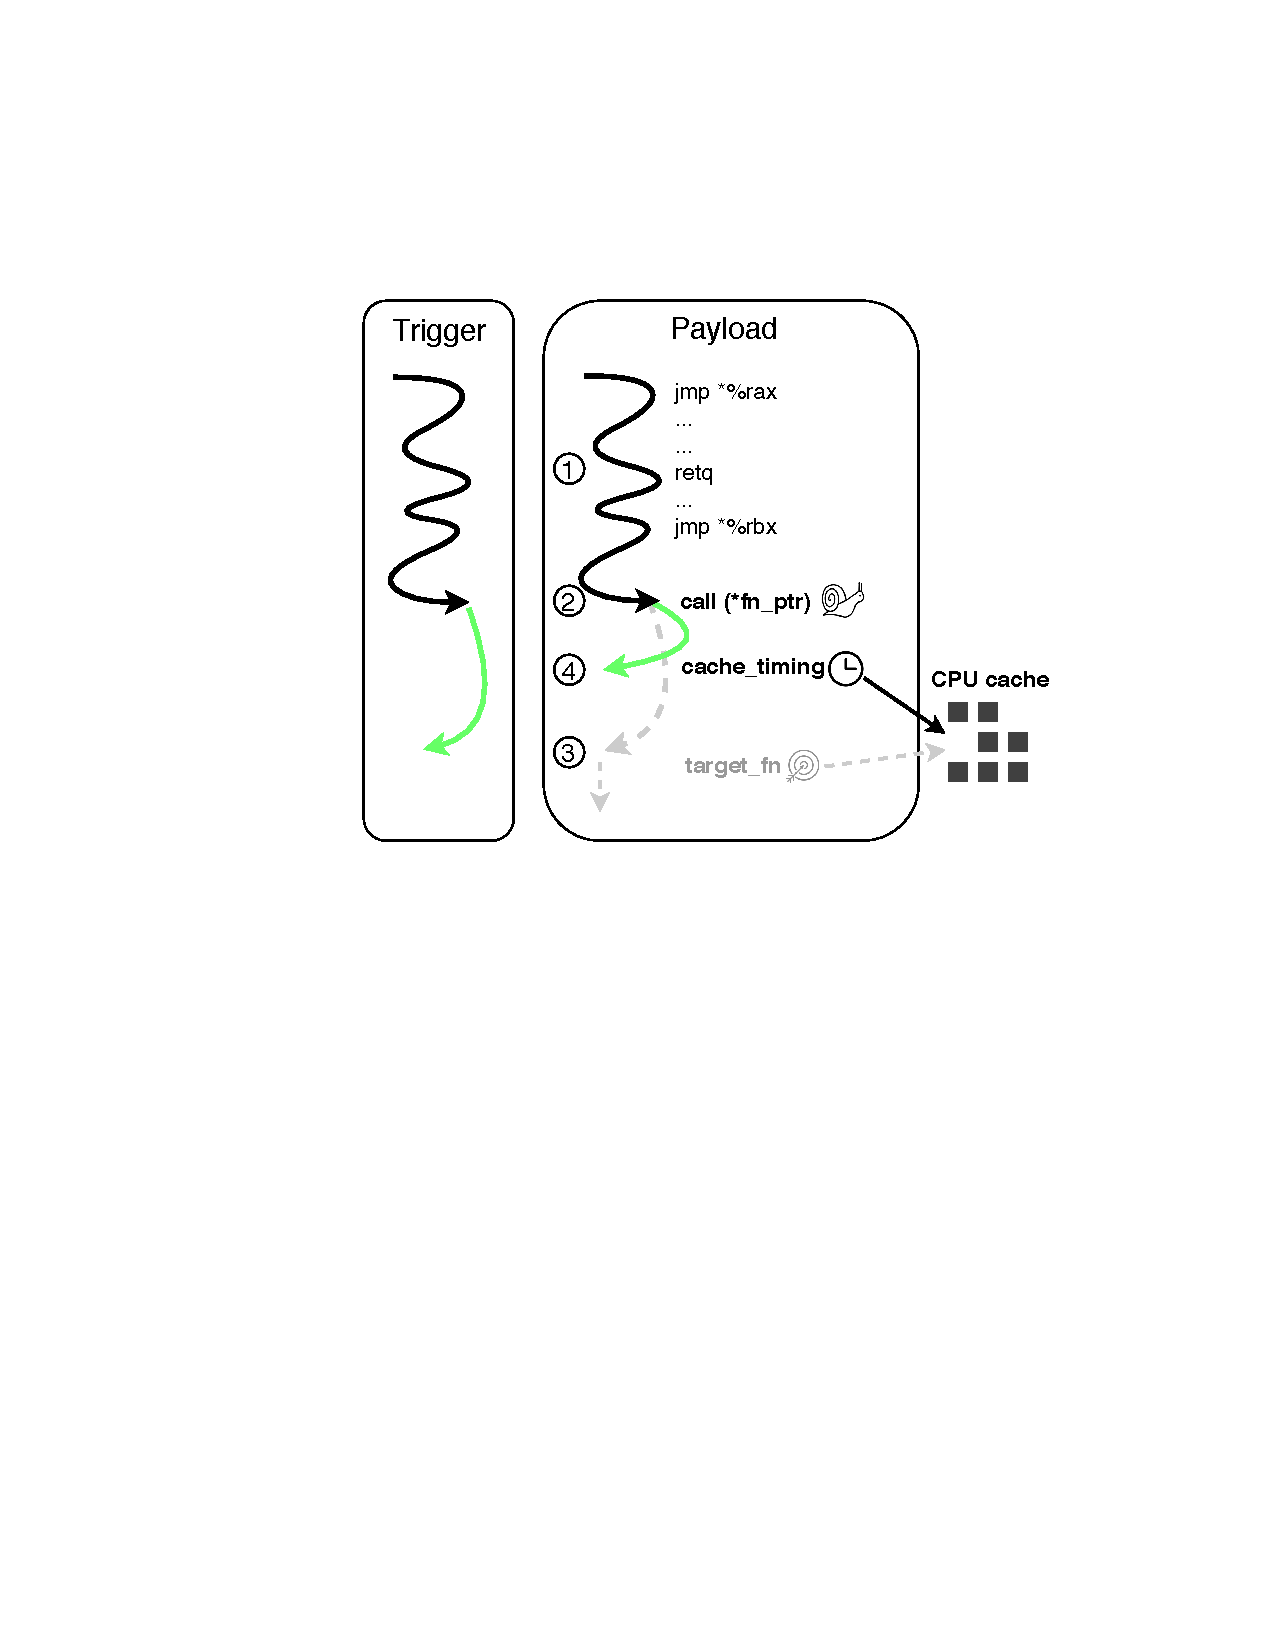
\includegraphics[clip, trim=6cm 13.5cm 3.8cm 5cm, width=0.9\linewidth]{figures/exspectre-high-level.pdf}
    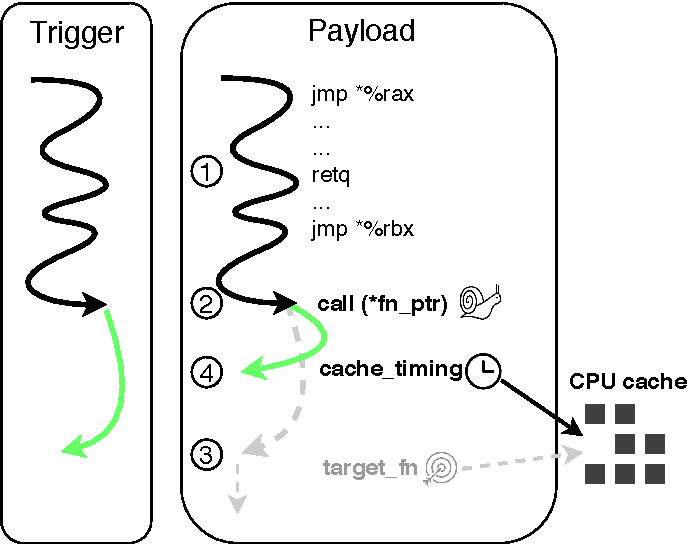
\includegraphics[width=0.9\linewidth]{figures/exspectre-high-level-trimmed.pdf}
    \caption{\textbf{Exspectre}\,---\, %
    1, 2, 3, 4...}

    \label{fig:high-level}

\end{figure}
}


\newcommand{\FigSpecMeasure}{
\begin{figure*}[t]
    \centering
        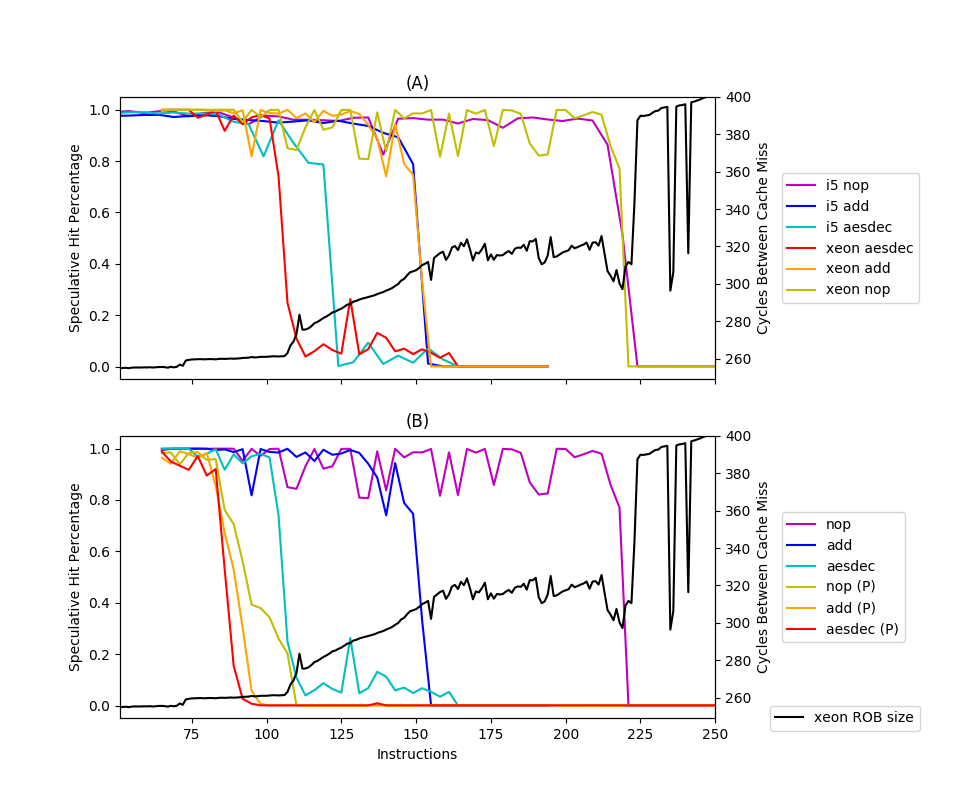
\includegraphics[width=0.9\textwidth]{figures/speculative_measurements.png}
    \caption{The speculative primitive allows for a limited number of instructions
        to be completed speculatively, dependent on multiple factors. A) The 
        processor generation determines the maximum ROB size and PRF capacity,
        however intel xeon E3-1270(warm colors) and i5-7200U both (cool colors) 
        perform similarly for comparable instructions. B) Because trigger and 
        payload processes must share cpu resources they must be performed on 
        the same hyperthread or associated parity hyperthreads. Processes on
        the parity hyperthreads (warm colors) denoted by (P) accomplish a 
        significantly lower number of instructions as compared with processes 
        on the same hyperthread (cool colors).}
    \label{fig:spec-capacity}
\end{figure*}
}

